\documentclass[landscape]{article}
\usepackage{tikz}
\usetikzlibrary{shapes,arrows,positioning}
\usepackage{geometry}

% Adjust the page layout with the geometry package
\geometry{left=2cm, right=2cm, top=2cm, bottom=2cm}

\begin{document}
\begin{figure}
    \centering
    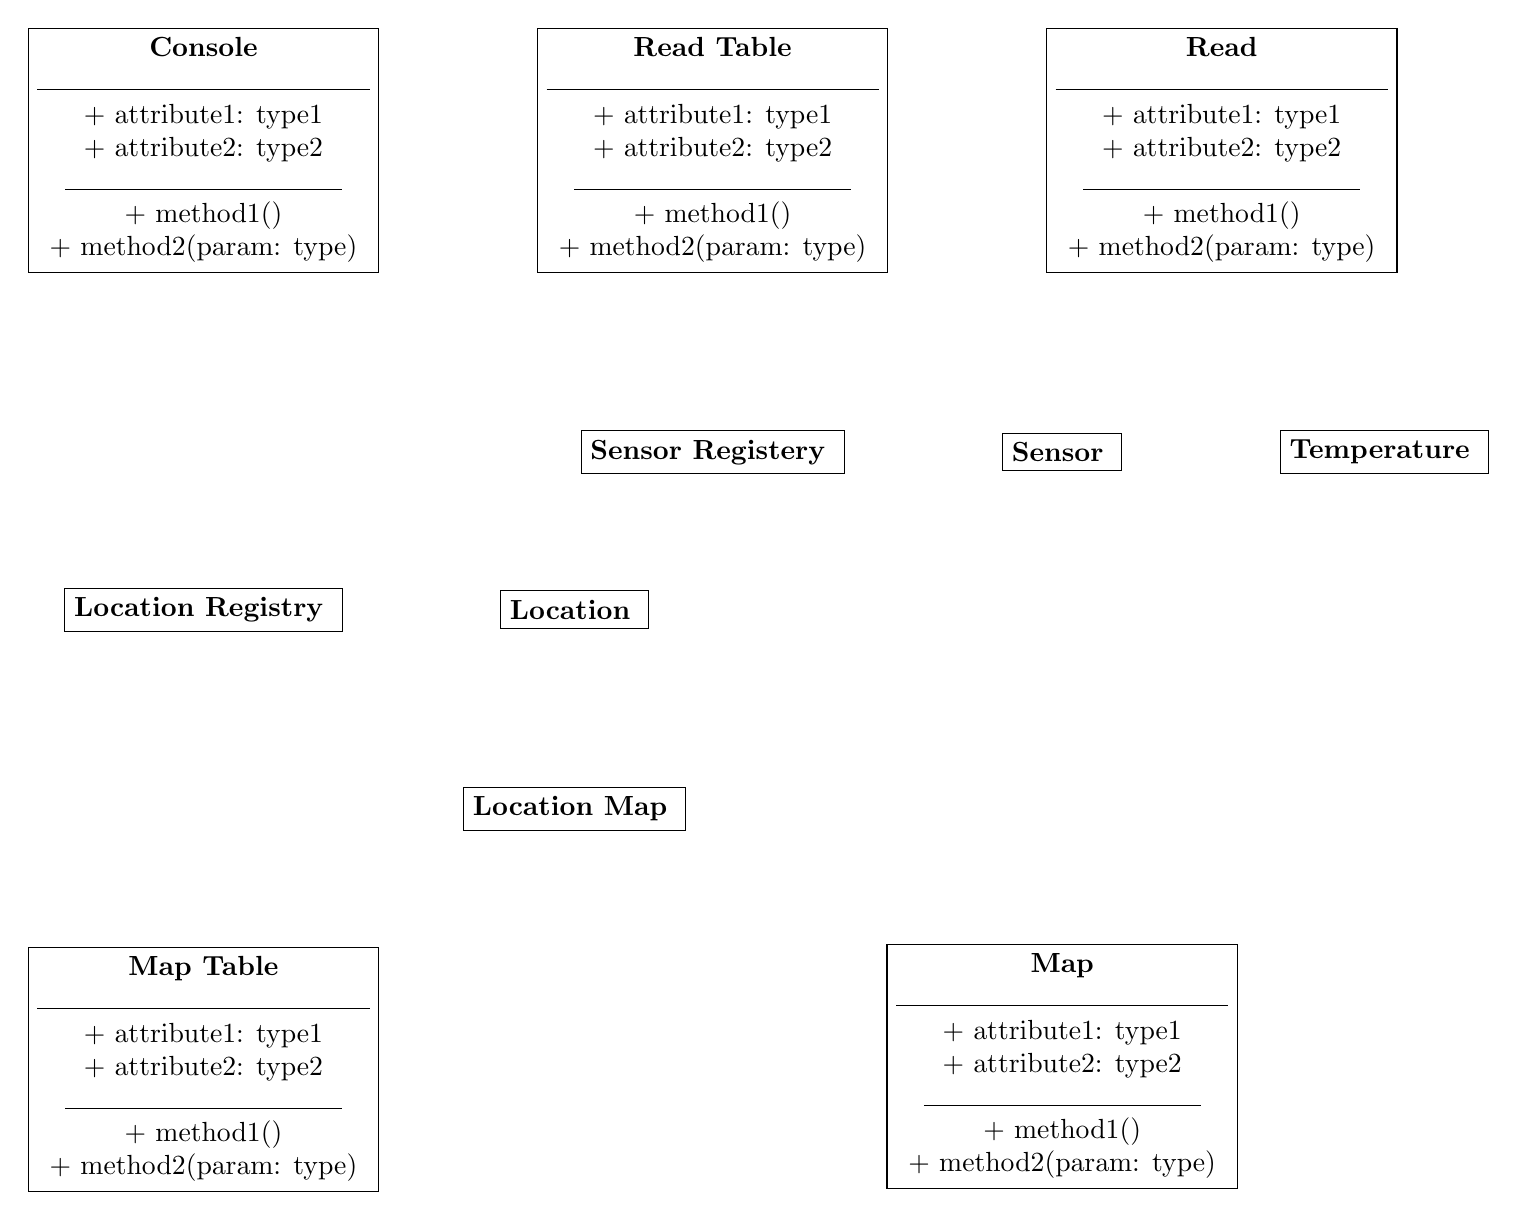
\begin{tikzpicture}
    
    	%-----Classes-----
        % Console Class
        \node [rectangle, draw, align=center] (console) {%
            \textbf{Console} \\
            \line(1,0){120} \\
            + attribute1: type1 \\
            + attribute2: type2 \\
            \line(1,0){100} \\
            + method1() \\
            + method2(param: type)
        };
        
        % Location Registry Class
        \node [rectangle, draw, below=4cm of console, align=center] (lreg) {%
            \textbf{Location Registry}
        };
        
        % Read Table Class
        \node [rectangle, draw, right=2cm of console, align=center] (readt) {%
            \textbf{Read Table} \\
            \line(1,0){120} \\
            + attribute1: type1 \\
            + attribute2: type2 \\
            \line(1,0){100} \\
            + method1() \\
            + method2(param: type)
        };
		
		 % Read Class
        \node [rectangle, draw, right=2cm of readt, align=center] (read) {%
            \textbf{Read} \\
            \line(1,0){120} \\
            + attribute1: type1 \\
            + attribute2: type2 \\
            \line(1,0){100} \\
            + method1() \\
            + method2(param: type)
        };
        
         % Sensor Registry Class
        \node [rectangle, draw, below=2cm of readt, align=center] (sreg) {%
            \textbf{Sensor Registery} 
        };
        
        % Sensor Class
        \node [rectangle, draw, right=2cm of sreg, align=center] (sensor) {%
            \textbf{Sensor} 
        };
       
       % Temperature Class
        \node [rectangle, draw, right=2cm of sensor, align=center] (temp) {%
            \textbf{Temperature} 
        };
        
        % Location Class
        \node [rectangle, draw, right=2cm of lreg, align=center] (loc) {%
            \textbf{Location} 
        };
        
        % Location Map Class
        \node [rectangle, draw, below=2cm of loc, align=center] (locmap) {%
            \textbf{Location Map} 
        };
        
        % Map Table Class
        \node [rectangle, draw, below=4cm of lreg, align=center] (mapt) {%
            \textbf{Map Table}  \\
            \line(1,0){120} \\
            + attribute1: type1 \\
            + attribute2: type2 \\
            \line(1,0){100} \\
            + method1() \\
            + method2(param: type)
        };
        
         % Map Class
        \node [rectangle, draw, below=6cm of sensor, align=center] (map) {%
            \textbf{Map}  \\
            \line(1,0){120} \\
            + attribute1: type1 \\
            + attribute2: type2 \\
            \line(1,0){100} \\
            + method1() \\
            + method2(param: type)
        };
        
        
    \end{tikzpicture}
    \caption{UML Class Diagram for Sensor System}
\end{figure}
\end{document}
